%%%%%%%%%%%%%%%%%%%%%%%%%%%%%%%%%%%%%%%%%%%%%%%%%%%%%%%%%%%%%%%%%%%%%%%%%%%%%%%%%%%%%%%%%%%%%%%%%%%%%%
%
%   Filename    : chapter_3.tex 
%
%   Description : This file will contain your Research Methodology.
%                 
%%%%%%%%%%%%%%%%%%%%%%%%%%%%%%%%%%%%%%%%%%%%%%%%%%%%%%%%%%%%%%%%%%%%%%%%%%%%%%%%%%%%%%%%%%%%%%%%%%%%%%

\chapter{Pipeline}
This chapter contains procedures that propoenents will follow for the research based from theories and concepts discussed in chapter 3 and the methodologies discussed in chapter 1.

\section{Data Collection}

In this phase, the proponents expanded the original music dataset for SOMphony. Each of the 5 eras now has 5 composers with 5 symphonies each. This sums up to a total of 125 symphonies. The proponents have also decided to only include composers that have composed at least 5 symphonies to be able to maintain a balanced data set. The process of selecting which symphonies to be added would be by random to have a better grasp of the general style of the composer. The audio files were retrieved from online sources and physical means. The researchers did not take into consideration the file type and bitrate of the audio files since music data that is free for use is limited.

\section{Data Preprocessing}
The audio files were trimmed using Audacity, removing the silent parts usually found at the start and/or end of the composition. This would reduce the amount of empty data, since no features can be extracted when there is no audio. After the music files were trimmed, they will be cut into one second music segments with a half-second overlap as discussed in Section 1.5.3 using Direct WAV MP3 Splitter.

\section{Feature Extraction}
The music segments then had their features extracted using jAudio, producing an XML file as an output. The proponents have decided to extract 436 features, refer to Appendix C for the complete list with their descriptions. All the features that don’t have variable-sized dimension were the ones selected. The XML file will then be converted into CSV format. The result would be a CSV file containing all the features determined for each segment. The proponents would then run a RegEx script from SOMphony to extract the unnecessary text in preparation for labeling. The data needs to be labeled according to their composer, composition and file name.

\section{Feature Selection}
In this phase, the proponents trimmed down the 436 features that jAudio has extracted to lessen the training time for the SOM. Since a lot of features were already reduced in the jAudio step through the removal of columns with entire 0 values and columns with at least a single NaN value, this leaves a total of only 276 features with values that have actual relevant values. Principal component analysis was further used to reduce the number of features by merging columns that have similar data thereby limiting the components to 50. The dataset finally resulted with the top 50 features while still retaining the essence of the original data.

\section{t-SNE}
T-SNE was performed on the processed dataset by using the tool provided by Python’s sklearn following Maaten \& Hiton (2008)\'s concept. After which, the resulting points of one second music segment, with a total of 330777, were further processed with k-means clustering to be able to perform quantitative comparisons. Using the elbow method, with the horizontal axis being the values of k and the vertical axis being the sum of squared errors, the minimum SSE  was computed. In minimizing the SSE, it was concluded that k=5 would be the best k as shown in Figure 4.1 and after performing k-means clustering, the resulting points with their corresponding cluster label were extracted and was used to perform pairwise string comparisons for all the symphonies using different metrics. Since t-SNE produced good results and had the same purpose as SOM, the proponents decided to focus more on t-SNE instead of SOM due to the faster processing time.

\begin{figure}[H]
\caption{Elbow Method Result}
\centering
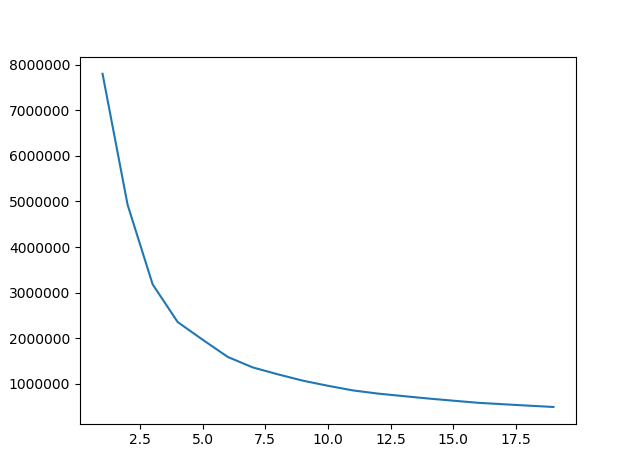
\includegraphics[scale=0.5]{elbow_method}
\end{figure}

\section{Distance Metrics}
Different metrics for comparing symphonies’ similarities pair-wise such as Levenshtein Distance, Damerau-Levenshtein Distance, Longest Common Subsequence, Manhattan Distance were used and the results are tabulated in chapter 5 for further analysis and discussion. For each metric, the comparisons were made via two methods, one using the unchanged number of points (330777), which shall be referred to as "Original" and the other, being only the transitions, which shall be called "Compressed"the  and this was done by compressing points with similar cluster labels and simply getting their centroid to represent the entirety of the compressed points. In this way, we can also see if simply comparing transitions would be a good enough tool for comparison compared to using the full length of points of each symphony produced by t-SNE.

\section{Visualization}
The proponents will visualize the data from t-SNE in 3D by plotting each point on a 2D plane and then collating the results of all segments within a symphony in time series. The result is a line $T (x, y, z)$ where $(x, y)$ denotes the coordinates of each point generated by t-SNE representing a specific music segment and $z$ being the index of the segment in the time series. Displaying the data of one symphony will plot a line that represents the musical trajectory or progression of the symphony from start to finish.

\begin{figure}[H]
\caption{Each point along the z-axis (longest axis) represents the position of a one second segment of a symphony in the time series.}
\centering
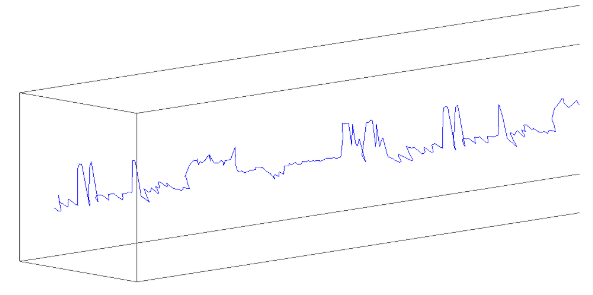
\includegraphics[scale=0.5]{3d1}
\end{figure}

\begin{figure}[H]
\caption{Overlaying the trajectories of two symphonies.}
\centering
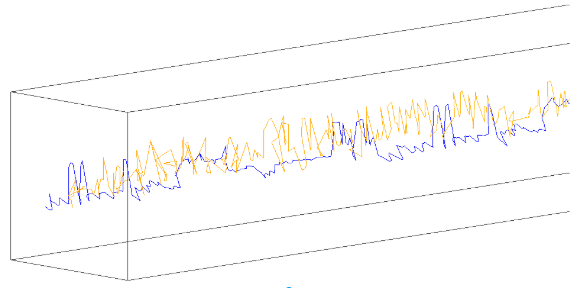
\includegraphics[scale=0.5]{3d2}
\end{figure}

\begin{figure}[H]
\caption{Colored ribbon to help visualize result of point-to-point comparison metrics. Green means close while red means far.}
\centering
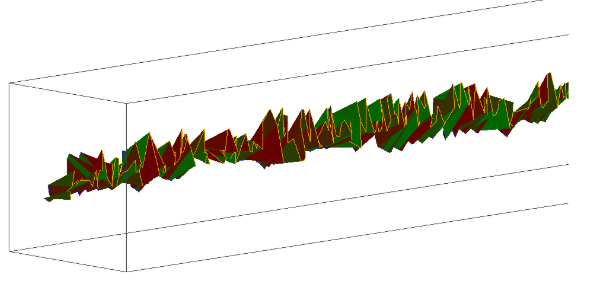
\includegraphics[scale=0.5]{3d3}
\end{figure}

Alternatively, an additional line can be generated to represent the musical trajectories of additional symphonies. By overlaying the trajectories of two different symphonies, it is possible to view the trajectories of multiple symphonies relative to each other. In addition, by drawing a plane between the trajectories and color coding the results, point-to-point comparison metrics such as Manhattan Distance can be visualized.